\documentclass[MsThesis, oneside]{thesis}
%Change to oneside or twoside based on what you need

\usepackage[total={16cm,24cm},includehead=true]{geometry}
%\captionsetup[table]{belowskip=4pt,aboveskip=4pt}
\usepackage{float}
\usepackage{array}
\newcolumntype{C}[1]{>{\centering\let\newline\\\arraybackslash\hspace{0pt}}m{#1}}
\usepackage{listings} 
\usepackage[linesnumbered,ruled]{algorithm2e}
\usepackage{algorithmic}			% for writing algortihm and psudo-codes	


\SetAlgorithmName{الگوریتم}{الگوریتم}{لیست الگوریتم‌ها}

\usepackage{setspace}

\usepackage{subfigure}
\usepackage[colorlinks=true]{hyperref}
\usepackage{xparse}
\usepackage{fancyhdr}
 
\renewcommand{\chaptermark}[1]{
 \markboth{\thechapter-\ #1}{}}

 \NewDocumentCommand\cfigure{O{scale=1.0}mom}
{\begin{figure}[!h] 
  \centering 
  \includegraphics[#1]{figures/#2.pdf}
  \IfNoValueTF {#3}
    {\caption{#4}}
    {\caption[#3]{#4}} 
  \label{#2} 
\end{figure}}
\usepackage[nottoc]{tocbibind} %فهرست تصاویر و جداول در فهرست
\usepackage[subfigure]{tocloft}
\usepackage{hyperref}
\usepackage[xindy, toc]{glossaries} 
\usepackage[font=small,labelfont=bf]{caption}

\usepackage{tikz}
  \usetikzlibrary{arrows}
  \usetikzlibrary{automata}
\usepackage{color,colortbl}		% color tex and color table
\usepackage{amsmath,amssymb,amsfonts,bm}	% for writing advanced math formula
\usepackage{graphicx}
\usepackage{url}
\usepackage{multicol}
\usepackage{multirow}

\usepackage{xepersian}


\usepackage{amsfonts}

% ------------------ Seth Figure Path ----------------------
\graphicspath{{}{images/}{images/chap1/}{images/chap2/}{images/chap3/}{images/chap4/}{images/chap5/}}
% -------------- Some Definitions for math -----------------
\def\mathbi#1{\textbf{\em #1}}					% define italic bold command as \mathbi
\DeclareMathOperator*{\argmax}{arg\,max} 		% define argmax operator 
\DeclareMathOperator*{\argmin}{arg\,min}		% define argmin operator
\DeclareMathOperator*{\sgn}{sgn}


\renewcommand{\listfigurename}{فهرست شکل‌ها}
\renewcommand{\listtablename}{فهرست جدول‌ها}
%\renewcommand{\listalgorithmname}{فهرست جدول‌ها}

\settextfont[Scale=1.166666666666666]{XBNiloofar}

\renewcommand{\arraystretch}{1.5}
%\setdigitfont{IR Yas}

\SepMark{\lr{-}}
\usepackage{perpage} %the perpage package
\MakePerPage{footnote} %the perpage package command
\localisecommands
\hypersetup{ 
pdfmenubar=false, pdfstartview=FitH, pdfpagemode=FullScreen,colorlinks=true,linkcolor=blue, anchorcolor=green, citecolor=magenta, urlcolor=cyan, filecolor=magenta, pdftoolbar=true, pdfpagemode=UseOutlines,
}
%texlive\2012\texmf-dist\tex\latex\glossaries\base\glossaries.sty
%style=listgroup,nonumberlist



\newglossarystyle{mylistFa}{
\glossarystyle{list}
\renewenvironment{theglossary}{}{}
\renewcommand*{\glossaryheader}{}
\renewcommand*{\glsgroupheading}[1]{\section*{\glsgetgrouptitle{##1}} }
\renewcommand*{\glsgroupskip}{}
\renewcommand*{\glossaryentryfield}[5]     {\noindent\glstarget{##1}{##2}\dotfill \space ##3 \\}
\renewcommand*{\glossarysubentryfield}[6]{\glossaryentryfield{##2}{##3}{##4}{##5}{##6}}
}\newglossarystyle{mylistEn}{
\glossarystyle{list}
\renewenvironment{theglossary}{}{}
\renewcommand*{\glossaryheader}{}
\renewcommand*{\glsgroupheading}[1]{\LTR\section*{\glsgetgrouptitle{##1}}} 
\renewcommand*{\glsgroupskip}{}
\renewcommand*{\glossaryentryfield}[5]     {\RTL\noindent\glstarget{##1}{##3}\dotfill \space ##2 \\}
\renewcommand*{\glossarysubentryfield}[6]{\glossaryentryfield{##2}{##3}{##4}{##5}{##6}}
}
% تعریف دو نمونه واژه نامه
\newglossary[glg]{english}{gls}{glo}{واژه‌نامه انگلیسی به فارسی}
\newglossary[blg]{persian}{bls}{blo}{واژه‌نامه فارسی به انگلیسی}
% توسط این دستور واژه مورد نظر در متن، هر دو واژه نامه و پاورقی می آید.
\newcommand{\inpdic}[2]{
	\newglossaryentry{fa-#1}{type=persian,name={#1}, sort={#1},description={\lr{#2}}}\gls{fa-#1}\LTRfootnote{#2}
	\newglossaryentry{en-#1}{type=english,name={\lr{#2}}, sort={#2},description={#1}}\glsuseri{en-#1}
}
% توسط این دستور واژه مورد نظر در متن، هر دو واژه نامه  می آید.
\newcommand{\indic}[2]{
	\newglossaryentry{fa-#1}{type=persian,name={#1}, sort={#1},description={\lr{#2}}}\gls{fa-#1}
	\newglossaryentry{en-#1}{type=english,name={\lr{#2}}, sort={#2},description={#1}}\glsuseri{en-#1}
}
% توسط این دستور واژه مورد نظر فقط در هر دو واژه نامه  می آید.
\newcommand{\ingls}[2]{
	\newglossaryentry{fa-#1}{type=persian,name={#1}, sort={#1},description={\lr{#2}}}\glsuseri{fa-#1}
	\newglossaryentry{en-#1}{type=english,name={\lr{#2}}, sort={#2},description={#1}}\glsuseri{en-#1}
}


\newcommand{\BigO}[1]{\ensuremath{\operatorname{\mathcal{O}}\bigl(#1\bigr)}} %usage \BigO(n) -> O(n)

\makeglossaries
\glsdisablehyper

\newlength\mylenprt 
\newlength\mylenchp
\newlength\mylenapp
\renewcommand\cftpartpresnum{\partname~}
\renewcommand\cftchappresnum{\chaptername~}
\renewcommand\cftchapaftersnum{:}
\settowidth\mylenprt{\cftpartfont\cftpartpresnum\cftpartaftersnum}
\settowidth\mylenchp{\cftchapfont\cftchappresnum\cftchapaftersnum}
\settowidth\mylenapp{\cftchapfont\appendixname~\cftchapaftersnum}
\addtolength\mylenprt{\cftpartnumwidth}
\addtolength\mylenchp{\cftchapnumwidth}
\addtolength\mylenapp{\cftchapnumwidth}
\setlength\cftpartnumwidth{\mylenprt}
\setlength\cftchapnumwidth{\mylenchp} 
\makeatletter
\renewcommand{\cftfigpresnum}{شکل\space}
\setlength{\cftfignumwidth}{5em}
\renewcommand{\@makechapterhead}[1]{%
{\setlength{\parindent}{0pt}
\fontspec[Script=Arabic,Mapping=parsidigits,Scale=3]{XBNiloofar}
\vspace*{50pt}
\ifnum \value{secnumdepth}>1 
\if@mainmatter \rule{\textwidth}{1pt}\vspace{5pt}\\\vspace{5pt}\textbf{\@chapapp\space\thechapter}\offinterlineskip\\\rule{\textwidth}{1pt}\vspace{30pt}\\\ \fi%
\fi
\parbox{\linewidth}{\textbf{\fontspec[Script=Arabic,Mapping=parsidigits,Scale=2]{XBNiloofar} #1}}\par\nobreak\vspace{40 pt}}}
\renewcommand{\@makeschapterhead}[1]{%
{\setlength{\parindent}{0pt}
\fontspec[Script=Arabic,Mapping=parsidigits,Scale=3]{XBNiloofar}
\vspace*{50pt}
\parbox{\linewidth}{\textbf{\fontspec[Script=Arabic,Mapping=parsidigits,Scale=2.5]{XBNiloofar} #1}}\par\nobreak\vspace{40 pt}}}
\makeatother

\renewcommand{\bibname}{مراجع}
\makeatletter
\renewcommand{\@makefntext}[1]{\parindent 1em
   \noindent\hbox to 1em{}% if you want to indent footnote text you can change the width of the hbox (e.g. \hbox to 2em{})
   \llap{\if@RTL\else\latinfont\fi\@thefnmark.\,\,}#1}
\makeatother
%\numberwithin{algorithm}{chapter}
\begin{document}
\آرم{\درج‌تصویر{logo}}
\تاریخ{ بهار ۱۳۹۴}
\عنوان{دسته‌بندی ریزدانه‌ای تصاویر}
\نویسنده{یاسر سوری}
\دانشگاه{دانشگاه صنعتی شریف\\دانشکده مهندسی کامپیوتر}
\موضوع{‌هوش‌ مصنوعی}
\استادراهنما{دکتر شهره کسایی}

\تقدیم{\درشت تقدیم به }
\frontmatter \makethesistitle \pagestyle{empty}  \baselineskip1.2\baselineskip
\شروع{تصویب}
\داور{ممتحن داخلی}{دکتر محمد تقی منظوری شلمانی}
\داور{داور خارجی}{دکتر بابک نجار اعرابی}
\پایان{تصویب}
%
\شروع{قدردانی}
باعث افتخار بود که 
\پایان{قدردانی}
\شروع{چکیده}{بینایی کامپیوتری، بازشناسی شیء، یادگیری عمیق، دسته‌بندی تصاویر، بازشناسی ریزدانه‌ای} 
\baselineskip1.5\baselineskip
{\small\singlespacing\linespread{1.2}
دسته‌بندی تصویر ریزدانه‌ای عبارت است از }
\پایان{چکیده}
%\setstretch{baselinestretch}
%\baselineskip.66666666666666666667\baselineskip

\pagestyle{plain}\pagenumbering{tartibi}\tableofcontents\newpage\listoffigures\newpage\listoftables\newpage %\listofalgorithms\newpage

\mainmatter%\pagestyle{headings}
 \baselineskip1.5\baselineskip

\pagestyle{fancyplain}
 
\fancyhf{}
  \renewcommand{\chaptermark}[1]{\markboth{\chaptername\space\thechapter\space-\space#1}{}} 
\lhead{\fancyplain{}{\thepage}}
\rhead{\fancyplain{}{\leftmark}}
%%%%%%%%%%%%%%%%%%%%%%%%%%%%%%%%%%%%%%%%%%%%%%%%
%\pagestyle{headings}

\chapter{مقدمه}\label{chap:1}

%%%%%%%%%%%%%%%%%%%%%%%%%%%%%%%%%%%%%%
%            1.0
%%%%%%%%%%%%%%%%%%%%%%%%%%%%%%%%%%%%%%
البته چالش اصلی این مسئله تنوع تصاویر طبیعی است. این تنوع حاصل تفاوت در حالت
\LTRfootnote{Pose}
است. می توانید به شکل
\ref{fig:1:variation}
ارجاع دهید.

\begin{figure}
	\centering
	\subfigure[]{\label{fig:1:variation:obj}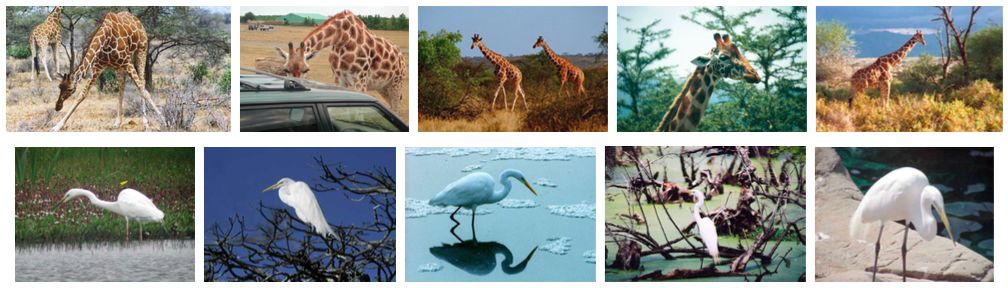
\includegraphics[width=0.9\textwidth]{var_obj}}
	\subfigure[]{\label{fig:1:variation:scene}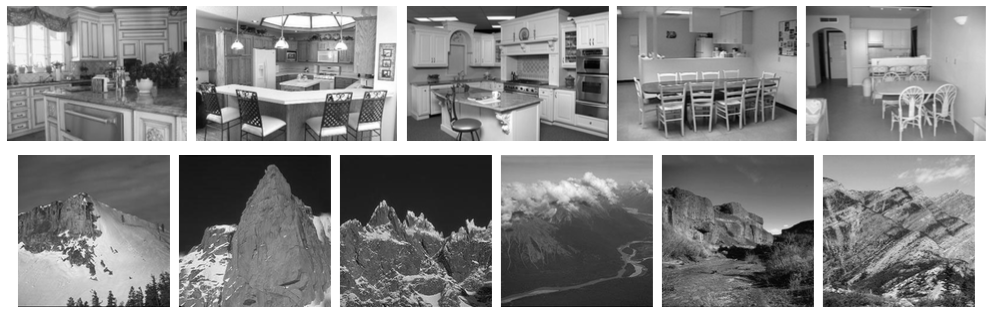
\includegraphics[width=0.9\textwidth]{var_scene}}
	\caption[نمونه‌هایی از انواع تنوع در تصاویر طبیعی که برای بازشناسی باید مورد توجه قرار بگیرد]{نمونه‌هایی از انواع تنوع در تصاویر طبیعی که برای بازشناسی باید مورد توجه قرار بگیرد\cite{phdlazeb}.
\subref{fig:1:variation:obj} اشیا معمولا به خاطر پوشیدگی و شلوغی به سختی قابل بازشناسی هستند. حیوانات از جمله اشیای غیر صلب هستند و در حالات مختلفی ظاهر می‌شوند.
\subref{fig:1:variation:scene} تصاویر صحنه‌های طبیعی مانند کوهستان دارای تفاوت درون دسته‌ای بسیار زیادی هستند. همچنین برخی تصاویر از محیط‌های داخلی (مانند آشپزخانه و اتاق نشیمن) به‌سختی از هم قابل تمایز هستند.}
	\label{fig:1:variation}
\end{figure}
\chapter{روش‌های پیشین}\label{chap:chap2}
%%%%%%%%%%%%%%%%%%%%%%%%%%%%%%%%%%%%%%
%            1.0
%%%%%%%%%%%%%%%%%%%%%%%%%%%%%%%%%%%%%%
در سال‌های اخیر پیشرفت‌های بسیار چشم‌گیری در زمینه‌ی دسته‌بندی تصویر رخ داده است.

%%%%%%%%%%%%%%%%%%%%%%%%%%%%%%%%%%%%%%
%            1.1
%%%%%%%%%%%%%%%%%%%%%%%%%%%%%%%%%%%%%%
\section{روش‌های دسته‌بندی تصویر}\label{chap:2:sec1}
همانطور که بیان شد، در دسته‌بندی تصویر، باید تصویر را با توجه به محتوایش دسته‌بندی کنیم.

\chapter{روش پیشنهادی}\label{chap:chap3}
روش پیشنهادی ...
\chapter{نتایج تجربی}\label{chap:chap4}

در این بخش به نتایج تجربی حاصل از پیاده‌سازی روش‌های معرفی شده در فصل
\ref{chap:chap3}
خواهیم پرداخت.
%%%%%%%%%%%%%%%%%%%%%%%%%%%%%%%%%%%%%%%%%%%%%%
%    4.1
%%%%%%%%%%%%%%%%%%%%%%%%%%%%%%%%%%%%%%%%%%%%%%
\section{معیار ارزیابی}
فرض کنید که داده‌های آزمایشی ما به صورت زوج مرتب‌های 
$ \Big\{ (x_i, y_i) \Big\}_{i=1}^{N_{test}} $
موجود باشد. که در آن $x_i$ تصویر، $y_i$ برچسب مربوط به آن و $N_{test}$ تعداد تصاویر آزمایشی است. همچنین در پایگاه داده پرندگان کلتک $N_{test}$ برابر با ۵۷۹۴ است.

حال برای ارزیابی تابع دسته‌بند یعنی
$ f(x) $
از فرمول

\begin{equation}
	mA = \frac{1}{\mathbb{C}} \sum_{c=1}^{\mathbb{C}} \frac{1}{|\alpha(c)|} \sum_{i \in \alpha(c)} \mathbb{I}(f(x_i) = y_i)
	\label{eq:4:ma}
\end{equation}
دقت میانگین را محاسبه می‌کنیم.


\section{نتایج نهایی روش پیشنهادی} \label{chap:4:final}

حالت دوم موسوم به DeepRF(All) که در آن روش پیشنهاد شده به غیر از مستطیل محیطی سر و بدن پرنده، لازم است که مستطیل محیطی کل پرنده را نیز تخمین بزند. به دلیل استفاده از جنگل تصادفی در این روش و ذات تصادفی بودن آن، آزمایش‌ها را سه بار انجام داده‌ایم و میانگین و انحراف معیار دقت را گزارش خواهیم کرد.

\begin{table}
	\centering
	\caption{دقت روش‌های نهایی پیشنهادی (مشخص شده توسط *) در مقایسه با روش مرز دانش. برای روش‌های پیشنهادی میانگین و انحراف معیار در سه آزمایش گزارش شده است.}
	\label{tbl:4:f_res}
	
	\footnotesize{
		\begin{tabular}{|c|c|c|c|c|c|C{2cm}|}
			\cline{3-6}
			\multicolumn{1}{r}{ }	&						&  \multicolumn{2}{c|}{آموزش} & \multicolumn{2}{c|}{آزمایش} \\
			\hline 	سال		&	نام					&	پنجره محیطی	&	مکان اجزا 	&	پنجره محیطی	&	مکان اجزا & 		دقت میانگین دسته‌بندی (درصد)	\\
			\hline 
			\hline 	2014 	& 	PRCNN \cite{partrcnn}	& \checkmark	& \checkmark	& \checkmark	& 			& 	76٫37				\\
			\hline 	- 		& 	DeepRF *				& \checkmark 	& \checkmark	&  \checkmark	& 			& 	73٫78 ($\pm$0٫32)		\\
			\hline
			\hline 	2014 	& 	PRCNN \cite{partrcnn}	& \checkmark	& \checkmark	& 			& 			& 	73٫89				\\
			\hline 	- 		& 	DeepRF(All) *			& \checkmark 	& \checkmark	& 			& 			& 	72٫02 ($\pm$0٫33)		\\
			\hline
		\end{tabular} 
	}
\end{table}

همانطور که در جدول
\ref{tbl:4:f_res}
نیز ذکر شده است، روش پیشنهادی موسوم به DeepRF به دقت میانگین 73٫78 دست پیدا می‌کند که قابل مقایسه با روش مرز دانش با دقت میانگین 76٫37 است. همچنین روش پیشنهادی موسوم به DeepRF(All) به دقت میانگین 72٫02 دست پیدا می‌کند. روش مرز دانش نیز به دقت میانگین 73٫89 درصد در حالتی که مستطیل محیطی در زمان آزمایش در دسترس نیست دست پیدا می‌کند.

به طور کلی می‌توان گفت که روش پیشنهاد شده از نظر کارایی بسیار سریع‌تر از روش مرز دانش است، از نظر سادگی بسیار ساده‌تر از آن است و از نظر کاربردی در موارد مختلف دیگری نیز با کمترین تغییرات می‌تواند مورد استفاده قرار بگیرد. با این حال از نظر دقت میانگین دسته‌بندی نتیجه‌ای بسیار نزدیک نسبت به آن کسب می‌کند.

\chapter{جمع‌بندی و کارهای آتی}\label{chap:chap5}

\section{جمع‌بندی}
در این پایان‌نامه به بررسی مسئله دسته‌بندی ریزدانه‌ای و اهمیت آن و همچنین روش‌های موجود برای حل آن پرداختیم. سپس دو روش جدید برای حل این مسئله بر روی پایگاه داده پرندگان کلتک پیشنهاد دادیم. 

\section{کارهای آینده}

\subsection{روشی برای }
یکی از محدودیت‌های روش پیشنهادی ...
%\chapter{جابجایی میانگین}\label{app:ms}
الگوریتم جابجایی میانگین روشی برای به دست آوردن ماکزیمم یک توزیع احتمال است که به روش ناپارامتری مدل شده‌ است \cite{Comaniciu2002}. در این روش مانند روش‌های مبتنی بر گرادیان، هدف به دست آوردن برداری است که با شروع از یک نقطه اولیه و حرکت در راستای آن به نقطه ماکزیمم یک توزیع ناپارامتری برسیم.
توزیع داده‌های $x_i$ را می‌توان به روش پنجره پارزن با هسته $k$به صورت زیر مدل کرد:
\begin{align}
\hat{f}_K(x) &= \frac{1}{nh^d} \sum_{i=1}^n k \Big( \|\frac{x-x_i}{h}\|^2 \Big)  \\
\nonumber g(x)&=-k'(x)
\end{align}
تخمین گرادیان توزیع احتمال فوق برابر است با:
\begin{align}
\nonumber  \hat{\bigtriangledown}f_K(x) \equiv \bigtriangledown \hat{f}_K(x) &= \frac{2}{nh^{d+2}} \sum_{i=1}^n (x-x_i) k' \Big(\ |\frac{x-x_i}{h}\|^2 \Big)  \\
\nonumber &= \frac{2}{nh^{d+2}} \sum_{i=1}^n (x_i-x) g \Big(\ |\frac{x-x_i}{h}\|^2 \Big)  \\
&= \frac{2}{nh^{d+2}} \Big[ \sum_{i=1}^n g \Big(\ |\frac{x-x_i}{h}\|^2 \Big) \Big] 
\Big[ \frac{\sum_{i=1}^n x_i g \Big(\ |\frac{x-x_i}{h}\|^2 \Big)}{\sum_{i=1}^n g \Big(\ |\frac{x-x_i}{h}\|^2 \Big)}-x \Big]
\label{equ:p1}
\end{align}
بردار جابجایی میانگین برابر عبارت زیر تعریف شده است:
\begin{equation}
M_{h,G}(x)=\frac{\sum_{i=1}^n x_i g \Big(\ |\frac{x-x_i}{h}\|^2 \Big)}{\sum_{i=1}^n g \Big(\ |\frac{x-x_i}{h}\|^2 \Big)}-x
\end{equation}
با جایگذاری $M_{h,G}(x)$ در رابطه \ref{equ:p1} داریم.
\begin{equation}
\hat{\bigtriangledown}f_K(x) = \hat{f}_G(x) \frac{2/C}{h^2} M_{h,G}(x)
\end{equation}
که در این رابطه  $\hat{f}_G$ تابع تخمین‌گر احتمال با هسته $G$ است. اکنون طبق رابطه فوق داریم.
\begin{equation}
M_{h,G}(x) = \frac{h^2}{2/C} \frac{\hat{\bigtriangledown}f_K(x)}{\hat{f}_G(x) }
\end{equation}
همان‌طور که انتظار می‌رفت این رابطه شبیه روش گرادیان است. در روش گرادیان برای ماکزیمم کردن یک تابع در راستای گرادیان آن حرکت می کردیم. در اینجا نیز بردار جابجایی میانگین  برحسب گرادیان به دست آمده، در واقع همان بردار گرادیان است که با $f_G$ نرمال شده است.
اکنون برای به دست آوردن ماکزیمم توزیع $\hat{f}_K$  طبق روش جابجایی میانگین باید رابطه بازگشتی زیر را محاسبه کنیم. 
\begin{equation}
y_{j+1}=\frac{\sum_{i=1}^n x_i g \Big(\ |\frac{y_j-x_i}{h}\|^2 \Big)}{\sum_{i=1}^n g \Big(\ |\frac{y_j-x_i}{h}\|^2 \Big)} \quad j=1,2,\ldots
\end{equation}
در  \cite{Comaniciu2002} ثابت شده که این  دنباله همگراست. حد دنباله فوق برابر ماکزیمم توزیع $\hat{f}_K$ است.
%\chapter{ویژگی هار} 
\label{app:haar}
در این بخش ویژگی هار به اختصار معرفی خواهد شد. این ویژگی در ابتدا برای بازیابی تصویر در   \cite{Tieu2004} استفاده شد و بعد از آن به دفعات در کاربردهای دیگر بینایی ماشین از آن استفاده شده است. 

برای  استخراج ویژگی هار مجموعه‌ای  از چندین فیلتر خطی مرتبه اول مانند شکل \ref{fig:linear-filters} در نظر می‌گیریم.
\begin{figure}[ht]
\centering
\includegraphics[width=7cm]{linear-filters}
\caption {\small {چند نمونه از فیلترهای خطی استفاده شده برای استخراج ویژگی}}
\label{fig:linear-filters}
\end{figure}
برای استخراج ویژگی از روی یک عکس به صورتی که در شکل \ref{fig:haar} نشان داده شده است تمامی این ۲۵ فیلتر با عکس مورد نظر کانولوشن و سپس \inpdic{نمونه‌برداری کاهشی}{Down-Sample} می‌شود. این کار تا سه مرحله انجام می‌شود و در نهایت میانگین رنگ پیکسل هرکدام از ۱۵۶۲۵ عکس به دست آمده در یکی از درایه‌های بردار ویژگی نهایی قرار می‌گیرد. 
\begin{figure}[ht]
\centering
\includegraphics[width=13cm]{haar}
\caption {\small {نمایش شماتیک نحوه استخراج ویژگی هار از روی عکس}}
\label{fig:haar}
\end{figure}
در این روش هدف از ترکیب فیلتر‌های ساده ساختن فیلترهایی است که ویژگی‌های خاصی از تصاویر را استخراج کنند مثلاً ترکیب سه فیلتر زیر، شکل \ref{fig:haar2} به نوارهای رنگی در شکل حساس بوده و مقدار بیشتری به عکس ببر اختصاص می‌دهد.
\begin{figure}
\centering
\includegraphics[width=5cm]{haar2}
\caption{\small {نتیجه اعمال فیلترهای مختلف بر روی دو عکس مختلف. همان طور که دیده می‌شود ترکیب این سه فیلتر به نوارهای رنگی حساس بوده و مقدار بیشتری به عکس ببر اختصاص می‌دهد.}}
\label{fig:haar2}
\end{figure}


%\PrepareForBiblio
%\begin{thebibliography}{1}
%\begin{LTRitems}
%\setpersianfont\bibitem{parsilatex}\resetlatinfont
%\newblock {\itshape ParsiLaTeX}.
%\newblock {http://parsilatex.com}
%\setpersianfont\bibitem{StBu}\resetlatinfont
%Stoer, J. and Bulirsch, R.
%\newblock {\itshape Introduction to numerical analysis},  Vol.~12 of {\itshape Texts in Applied Mathematics}.
%\newblock Springer-Verlag, New York, third Ed., 2002.
%\newblock Translated from the German by R. Bartels, W. Gautschi and C. Witzgall.
%\end{LTRitems}
%\end{thebibliography}



\footnotesize
%\bibliographystyle{ieeetr-fa}
%\bibliography{References}
\bibliographystyle{IEEEtran}

%%\bibliography{IEEEfull,References}

\vspace*{50pt}
{\LARGE{\textbf{مراجع}}}
\vspace{40pt}
\begin{latin}
\renewcommand{\chapter}[2]{}
\bibliography{IEEEabrv,References}  % sigproc.bib is the name of the Bibliography in 
\end{latin}
\baselineskip\baselineskip 

%\twocolumn{$ $}
%\LTRdblcol\twocolumn
%\glossarystyle{mylistEn}
%\addcontentsline{toc}{chapter}{واژه‌نامه}
%\printglossary[type=english]
%\clearpage
%\baselineskip2\baselineskip 
%\RTLdblcol\twocolumn
%\phantomsection
%\glossarystyle{mylistFa}
%\printglossary[type=persian]
%\onecolumn
%\baselineskip1.2\baselineskip
\PrepareForLatinPages

\date{Spring 2015}
\title{\sffamily ‫Fine-grained Image Classification}
\author{\sffamily Yaser Souri}
\university{Sharif University of Technology\\Department of Computer Engineering}
\subject{Artificial Intelligence}
\supervisor{\sffamily Prof. Shohreh Kasaei}

\begin{abstract}{Computer vision, Object recognition, Deep learning, Image classification, Fine-grained recognition}
{ %\small\singlespacing\linespread{1}
Fine-grained image classification is 
}
\end{abstract}
\makethesistitle
\end{document}
